LaTeX nimmt die *.tex Datei(en) und erstellt damit die eigentliche Druck-Datei (z.B. *.pdf). Dieser Vorgang ist nicht trivial. Abhängig von den gewünschten Ergebnissen resp. der zu erstellenden Verzeichnisse, muss der Übersetzungsvorgang mehrfach ausgeführt werden damit letztendlich das Dokument wie gewünscht erstellt wird.

Texmaker ist via \menu{Optionen > Texmaker konfigurieren} wie folgt zu konfigurieren:

\begin{figure}[h!]
\centering
  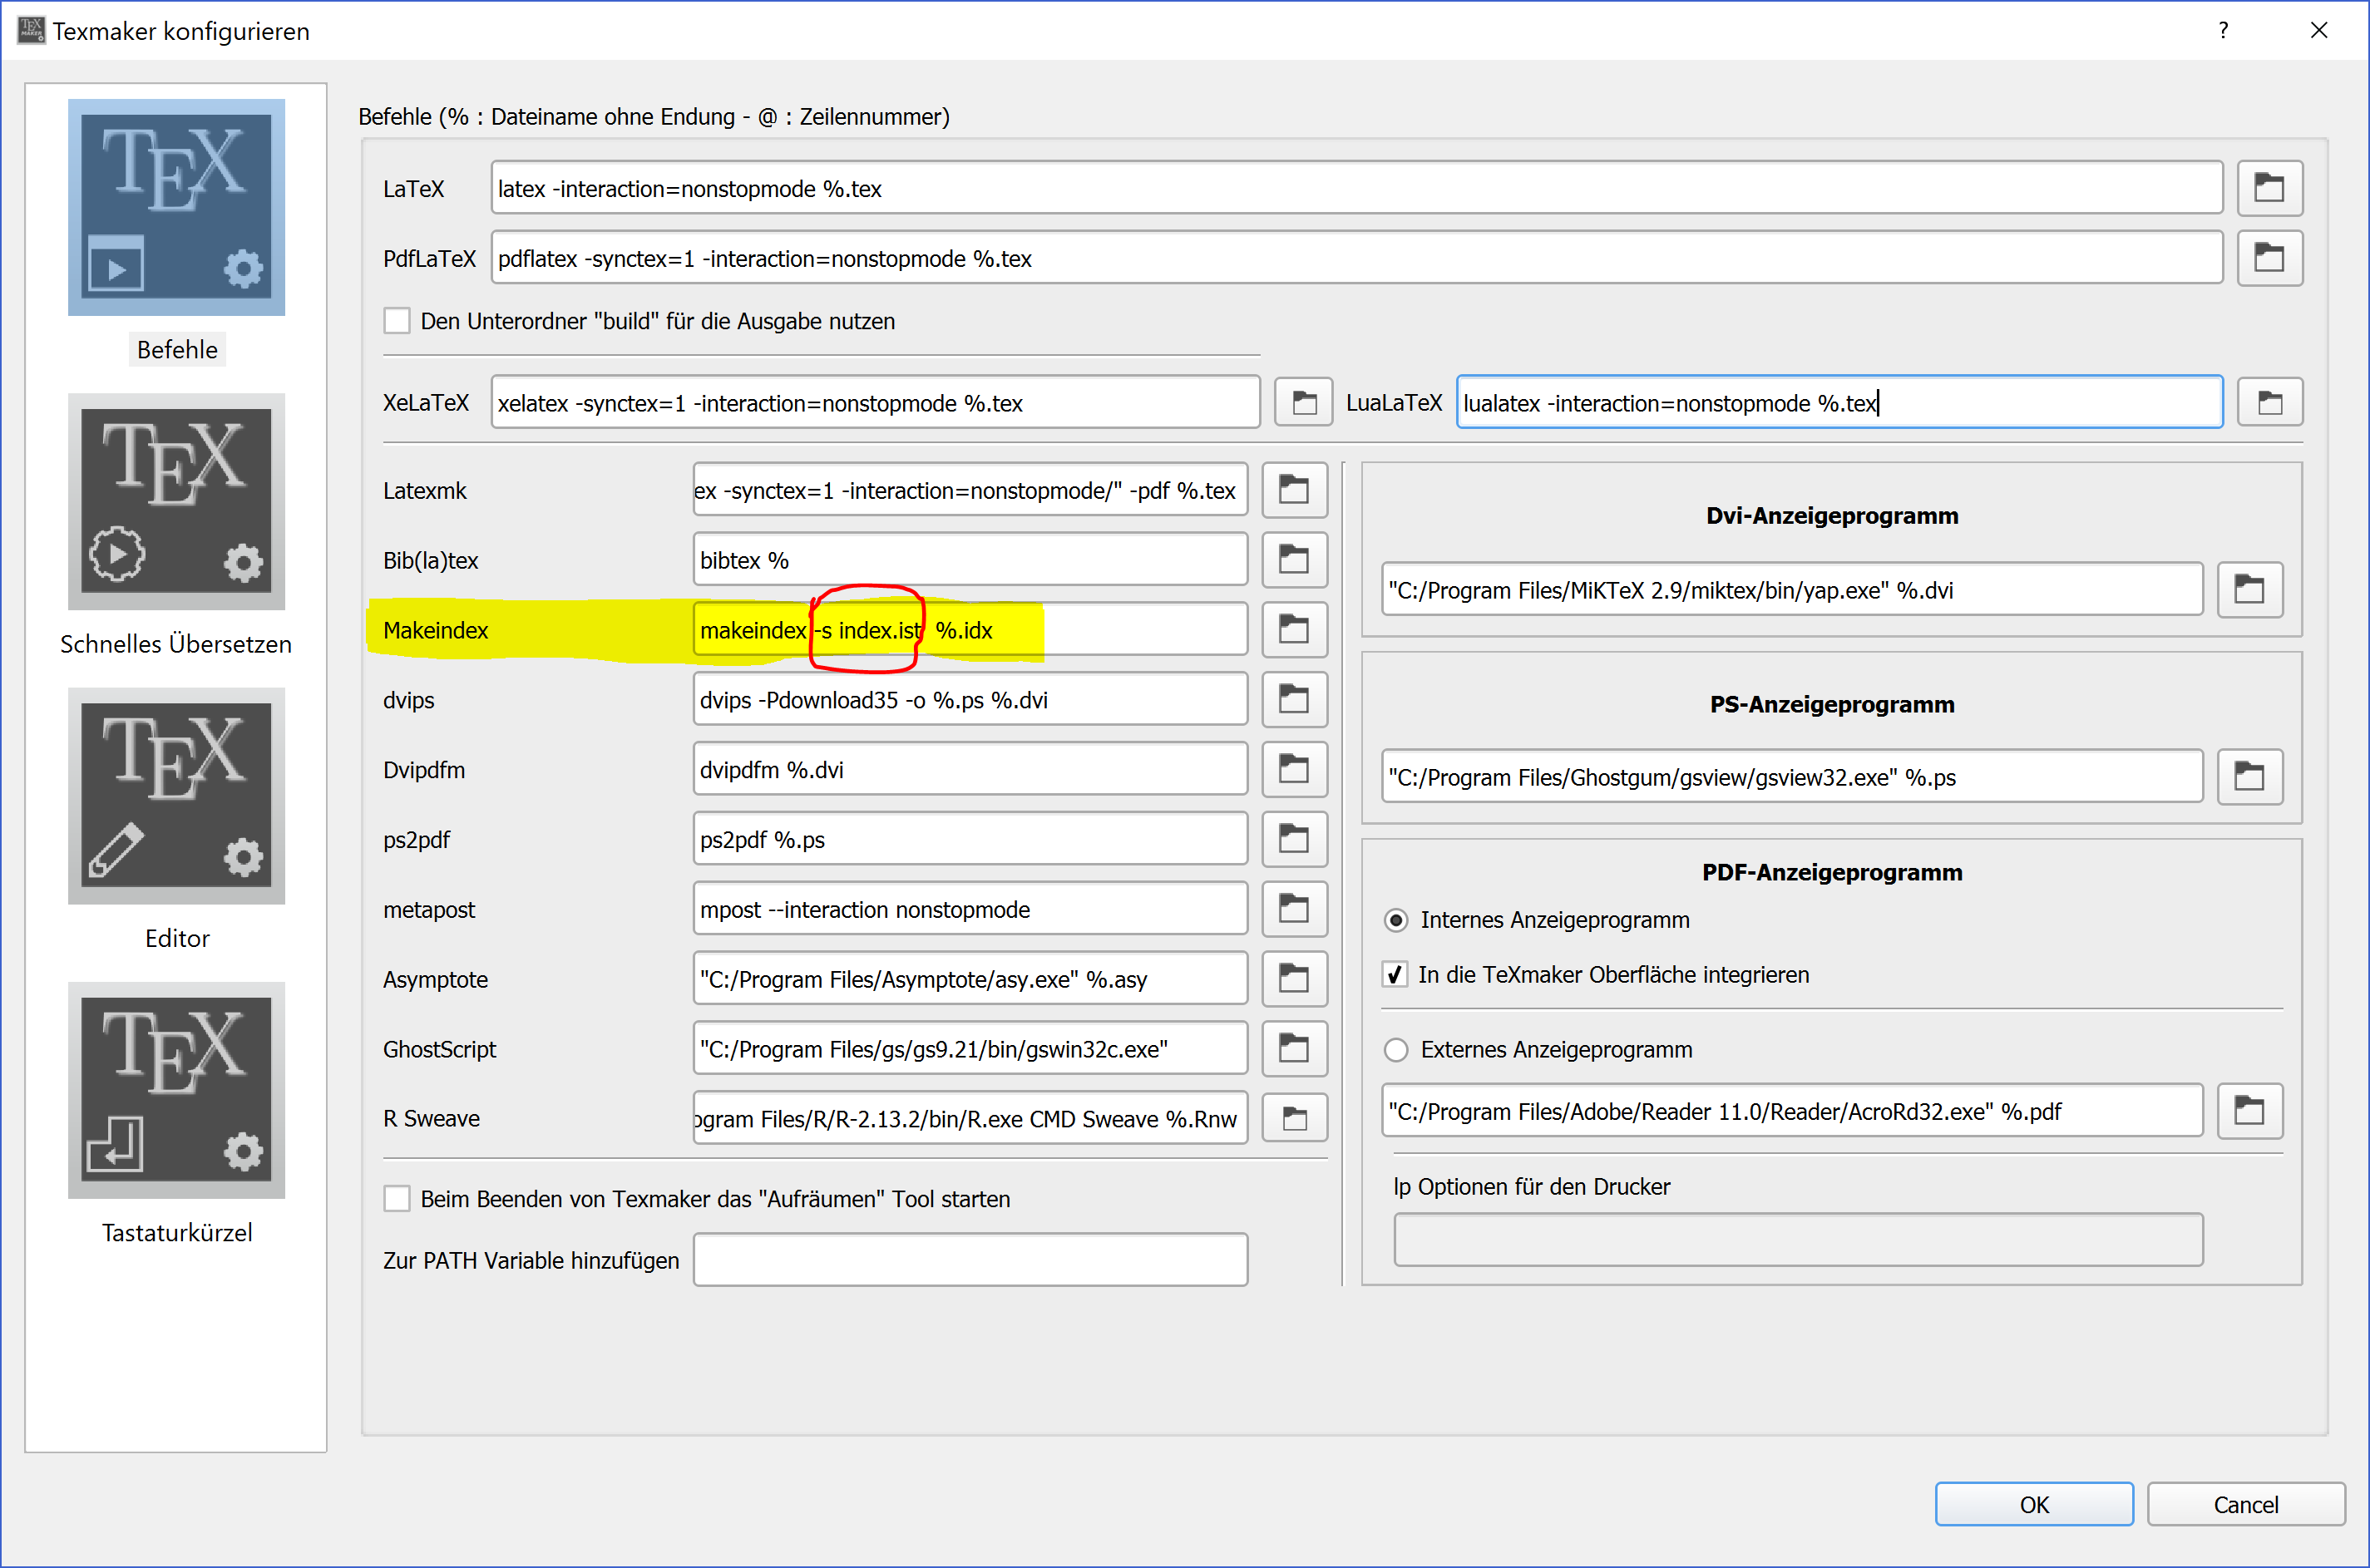
\includegraphics[width=0.6\textwidth]{./Bilder/Texmaker_Konfiguration_1.PNG}
  \caption{Konfiguration Latex: Befehle}
  \label{fig:Konfig}
\end{figure}

\begin{figure}[h!]
\centering
  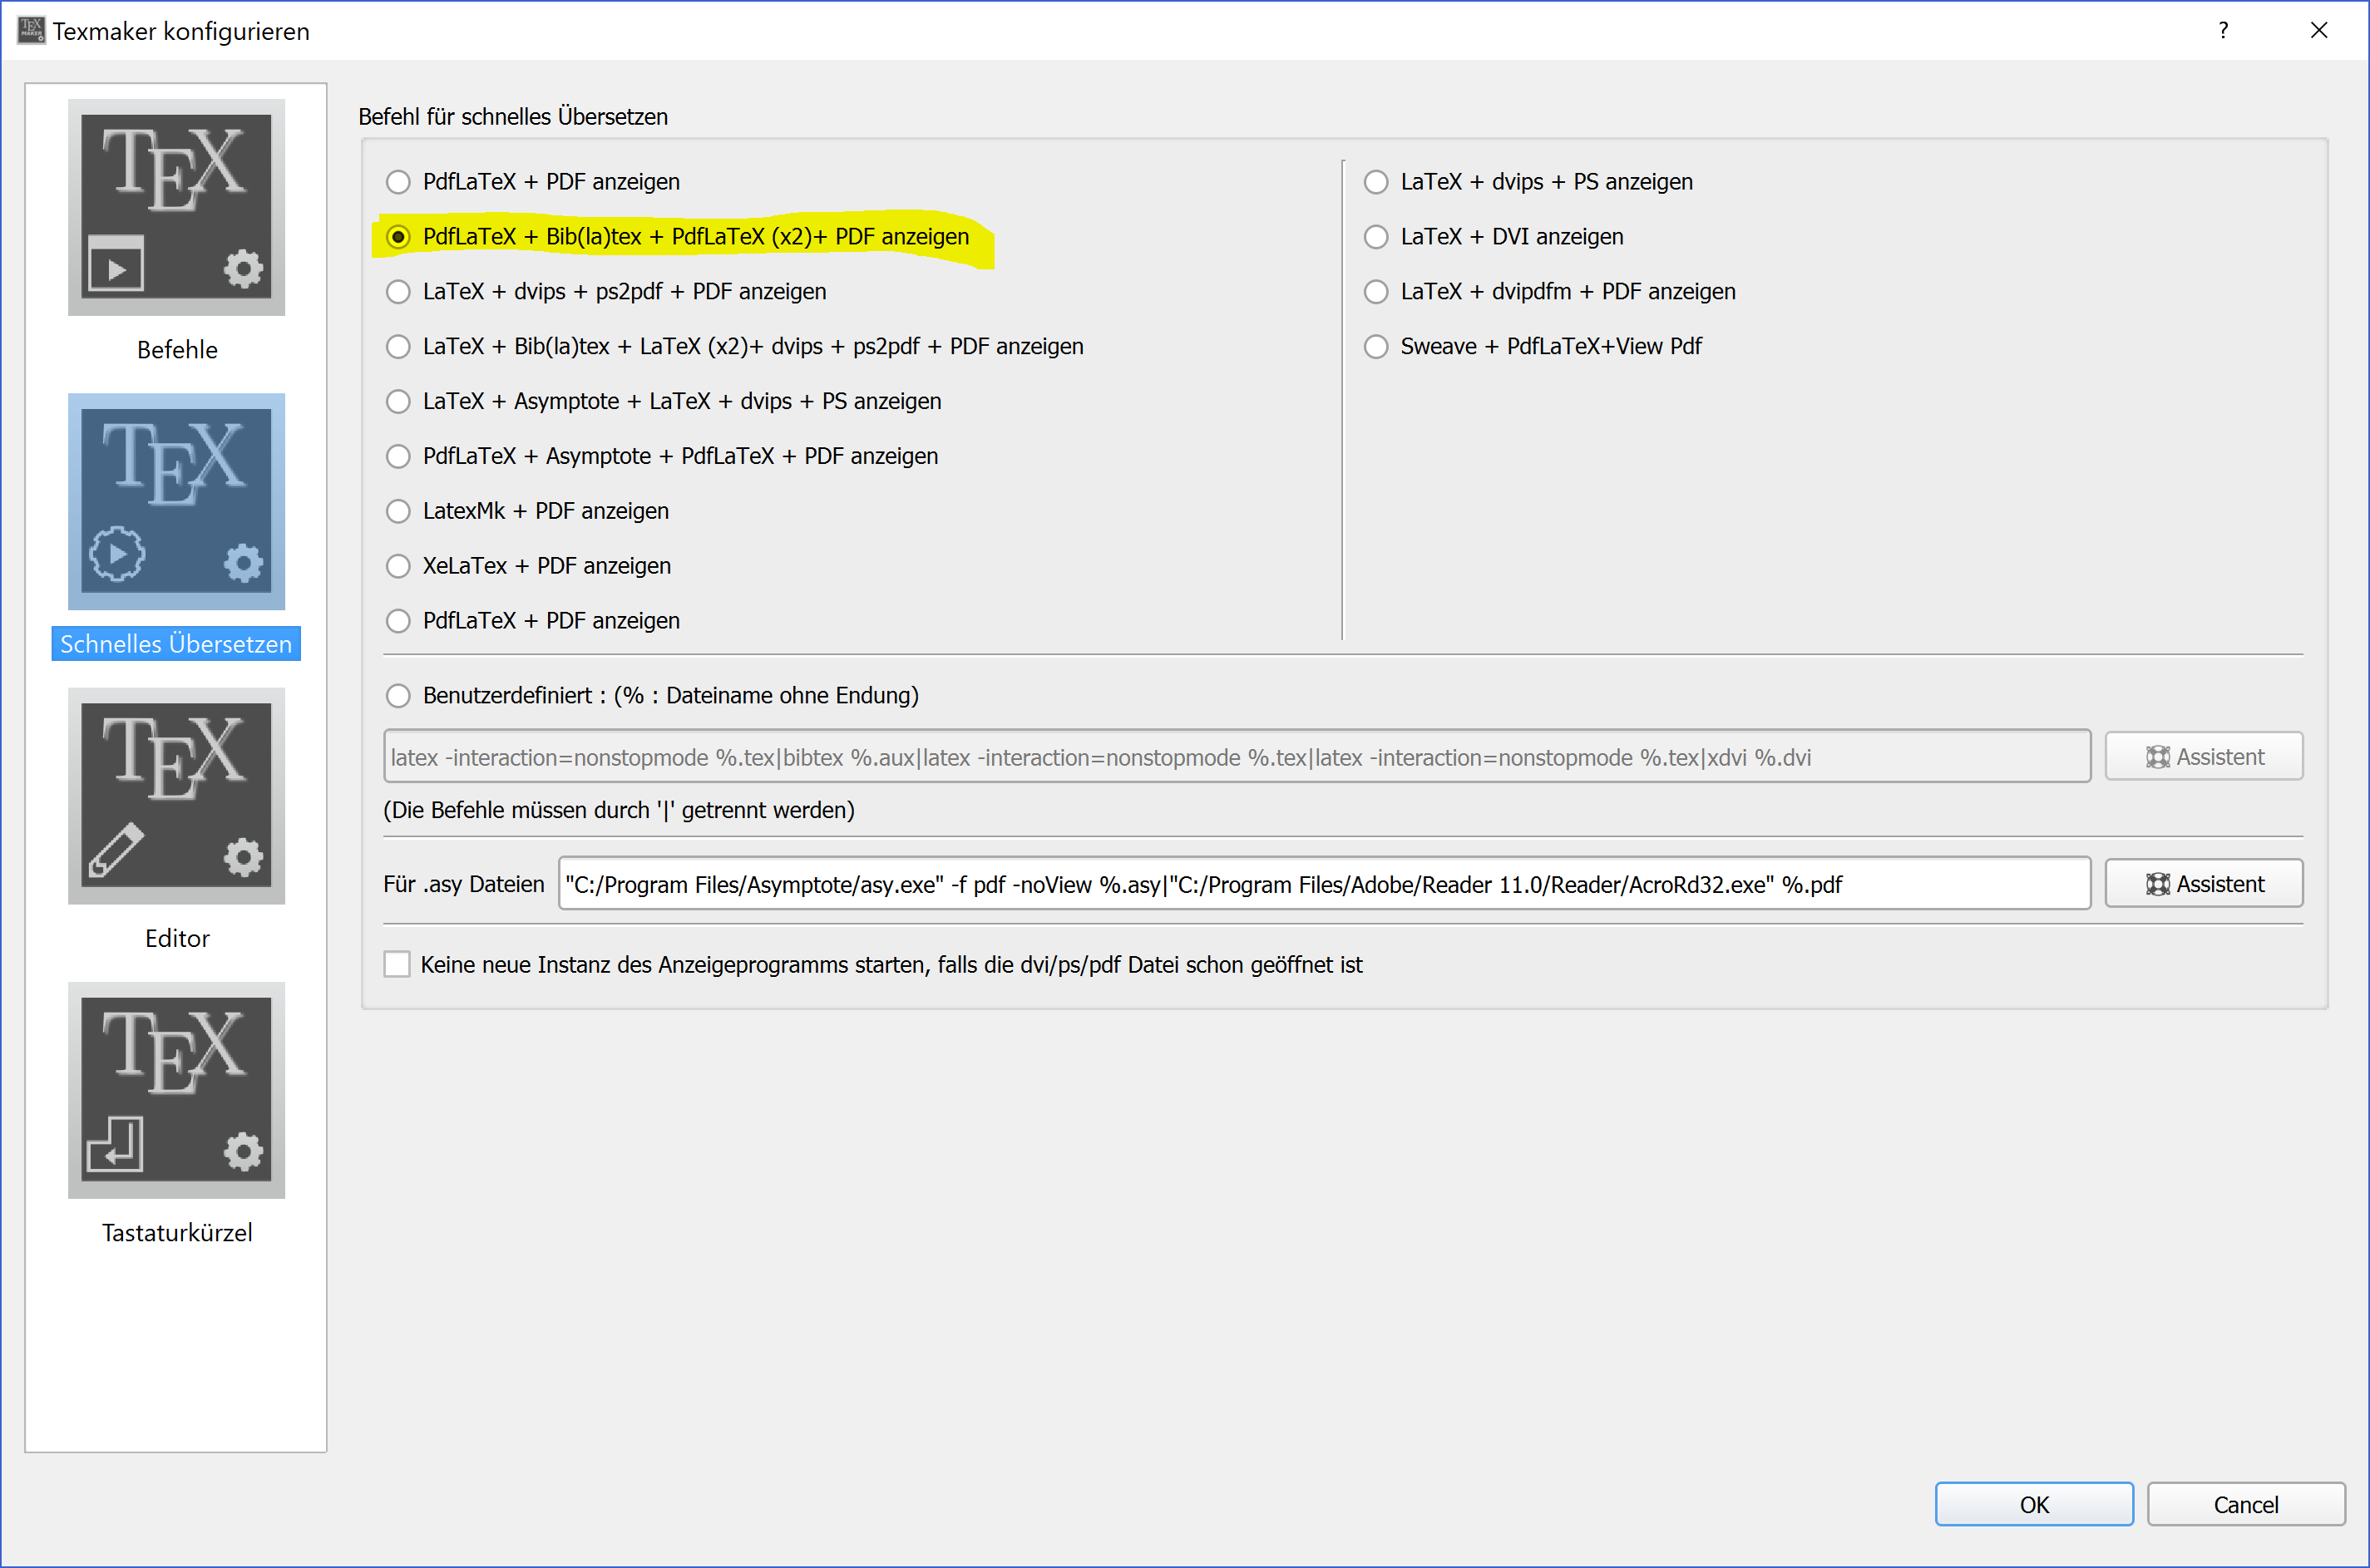
\includegraphics[width=0.6\textwidth]{./Bilder/Texmaker_Konfiguration_2.PNG}
  \caption{Konfiguration Latex: Schnelles Übersetzen}
\end{figure}

Zusätzlich muss dass Stichwortverzeichnis mit \keys{F12} manuell erstellt werden.

\textbf{\\Empfehlung:} 
\begin{quote}
Mit der Tasten-Folge \keys{F1} \keys{F12} \keys{F1} wird alles korrekt erstellt.
\end{quote}
